% ====== TAREA 3 MATEMATICAS APLICADAS ======
\documentclass{article}
\usepackage[utf8]{inputenc}
\usepackage[spanish]{babel}
\usepackage{amsmath, amsfonts, amssymb}
% \usepackage{ tipa }
\usepackage{graphicx}
\usepackage[usenames]{color}
\usepackage[text={20cm,25cm},centering,top=1.5cm,bottom=1.5cm,letterpaper,showframe=false]{geometry}
\renewcommand{\baselinestretch}{1.5}
\parindent  = 0mm
\parskip    = 4mm
\definecolor{azul}{RGB}{10,80,190}
\definecolor{negro}{RGB}{0,0,0}
\definecolor{rojo}{RGB}{190,80,10}
\definecolor{verde}{RGB}{0,120,50}

\begin{document}
    \title{Tarea-Examen 3}
    \author{Careaga Carrillo Juan Manuel\\
            Quiróz Castañeda Edgar\\
            Soto Corderi Sandra del Mar}
    \date{Viernes 7 de diciembre de 2018}
    \maketitle
    \begin{enumerate}

        % Ejercicio 1
        \item {
            Demostrar que

            \begin{enumerate}
            \item{
                $\nabla \times (f \mathbf{F}) =
                f \nabla \times \mathbf{F} + \nabla f \times \mathbf{F}$\\
                \color{azul}
            % Respuesta
                    Digamos que $\mathbf{F} = (f_1, f_2, f_3)$\\
                    Primero notemos que
                    \[\nabla \times \mathbf{F} =
                    \begin{bmatrix}
                        \hat{\imath} & \hat{\jmath} & \hat{k} \\
                        \frac{\partial}{\partial x} & \frac{\partial}{\partial y}
                         & \frac{\partial}{\partial z} \\
                         f_1 & f_2 & f_3
                    \end{bmatrix} =
                    (
                    \frac{\partial f_3}{\partial y}
                    - \frac{\partial f_2}{\partial z},
                    -\frac{\partial f_3}{\partial x}
                    +\frac{\partial f_1}{\partial z},
                    \frac{\partial f_2}{\partial x}
                    -\frac{\partial f_1}{\partial y}
                    )
                    \]
                    Y también que, como $\nabla f =
                    (\frac{\partial f}{\partial x},
                    \frac{\partial f}{\partial y}
                    \frac{\partial f}{\partial z})$

                    \[\nabla f \times \mathbf{F}\ =
                    \begin{bmatrix}
                        \hat{\imath} & \hat{\jmath} & \hat{k} \\
                        \frac{\partial f}{\partial x} &
                        \frac{\partial f}{\partial y}
                         & \frac{\partial f}{\partial z} \\
                         f_1 & f_2 & f_3
                    \end{bmatrix} =
                    (
                    f_3\frac{\partial f}{\partial y}
                    -f_2\frac{\partial f}{\partial z},
                    -f_3\frac{\partial f}{\partial x}
                    +f_1\frac{\partial f}{\partial z},
                    f_2\frac{\partial f}{\partial x}
                    -f_1\frac{\partial f}{\partial y}
                    )
                    \]
                    Entonces, como $f\mathbf{F} = f(f_1, f_2, f_3) =
                    (ff_1, ff_2, ff_3)$
                    \[
                    \nabla \times (f \mathbf{F}) =
                    \begin{bmatrix}
                        \hat{\imath} & \hat{\jmath} & \hat{k} \\
                        \frac{\partial}{\partial x} & \frac{\partial}{\partial y}
                         & \frac{\partial}{\partial z} \\
                         ff_1 & ff_2 & ff_3
                    \end{bmatrix} =
                    (
                    \frac{\partial ff_3}{\partial y}
                    - \frac{\partial ff_2}{\partial z},
                    -\frac{\partial ff_3}{\partial x}
                    +\frac{\partial ff_1}{\partial z},
                    \frac{\partial ff_2}{\partial x}
                    -\frac{\partial ff_1}{\partial y}
                    )
                    \]
                    Y por la regla del producto
                    \begin{align*}
                        &=
                        (
                        f_3\frac{\partial f}{\partial y}
                        +f\frac{\partial f_3}{\partial y}
                        -f_2\frac{\partial f}{\partial z}
                        -f\frac{\partial f_2}{\partial z},
                        -f_3\frac{\partial f}{\partial x}
                        -f\frac{\partial f_3}{\partial x}
                        +f_1\frac{\partial f}{\partial z}
                        +f\frac{\partial f_1}{\partial z},
                        f_2\frac{\partial f}{\partial x}
                        +f\frac{\partial f_2}{\partial x}
                        -f_1\frac{\partial f}{\partial y}
                        -f\frac{\partial f_1}{\partial y}
                        )\\
                        &=
                        (
                        f\frac{\partial f_3}{\partial y}
                        -f\frac{\partial f_2}{\partial z},
                        -f\frac{\partial f_3}{\partial x}
                        +f\frac{\partial f_1}{\partial z},
                        f\frac{\partial f_2}{\partial x}
                        -f\frac{\partial f_1}{\partial y}
                        )
                        +
                        (
                        f_3\frac{\partial f}{\partial y}
                        -f_2\frac{\partial f}{\partial z},
                        -f_3\frac{\partial f}{\partial x}
                        +f_1\frac{\partial f}{\partial z},
                        f_2\frac{\partial f}{\partial x}
                        -f_1\frac{\partial f}{\partial y}
                        )\\
                        &=f (
                        \frac{\partial f_3}{\partial y}
                        -\frac{\partial f_2}{\partial z},
                        -\frac{\partial f_3}{\partial x}
                        +\frac{\partial f_1}{\partial z},
                        \frac{\partial f_2}{\partial x}
                        -\frac{\partial f_1}{\partial y}
                        )
                        +
                        (
                        f_3\frac{\partial f}{\partial y}
                        -f_2\frac{\partial f}{\partial z},
                        -f_3\frac{\partial f}{\partial x}
                        +f_1\frac{\partial f}{\partial z},
                        f_2\frac{\partial f}{\partial x}
                        -f_1\frac{\partial f}{\partial y}
                        )
                    \end{align*}
                    Y por las dos igualdades notadas al inicio del ejericio,
                    esto es
                    \[ = f (\nabla \times \mathbf{F}) + \nabla f \times \mathbf{F}\]
            }

            \item{
            	$\nabla \times (\nabla \times \mathbf{F}) = \nabla (\nabla \cdot \mathbf{F}) - \nabla^2 \mathbf{F}$

           \color{azul}
            % Respuesta
                Por lo notado en el ejericio 1, tenemos que, con
                $\mathbf{F}=(f_1, f_2, f_3)$
                \[
                \nabla \times \mathbf{F} =
                (
                \frac{\partial f_3}{\partial y}
                - \frac{\partial f_2}{\partial z},
                -\frac{\partial f_3}{\partial x}
                +\frac{\partial f_1}{\partial z},
                \frac{\partial f_2}{\partial x}
                -\frac{\partial f_1}{\partial y}
                )
                \]
                Por lo que
                \begin{align*}
                    \nabla \times (\nabla \times \mathbf{F})
                    &= \nabla \times
                    (
                    \frac{\partial f_3}{\partial y}
                    - \frac{\partial f_2}{\partial z},
                    -\frac{\partial f_3}{\partial x}
                    +\frac{\partial f_1}{\partial z},
                    \frac{\partial f_2}{\partial x}
                    -\frac{\partial f_1}{\partial y}
                    )\\
                    &=
                    (
                    \frac{\partial (\frac{\partial f_2}{\partial x}
                    -\frac{\partial f_1}{\partial y})}{\partial y}
                    - \frac{\partial (-\frac{\partial f_3}{\partial x}
                    +\frac{\partial f_1}{\partial z})}{\partial z},
                    -\frac{\partial (\frac{\partial f_2}{\partial x}
                    -\frac{\partial f_1}{\partial y})}{\partial x}
                    +\frac{\partial (\frac{\partial f_3}{\partial y}
                    - \frac{\partial f_2}{\partial z})}{\partial z},
                    \frac{\partial (-\frac{\partial f_3}{\partial x}
                    +\frac{\partial f_1}{\partial z})}{\partial x}
                    -\frac{\partial (\frac{\partial f_3}{\partial y}
                    - \frac{\partial f_2}{\partial z})}{\partial y}
                    )\\
                    &=
                    (
                    \frac{\partial^2f_2}{\partial x \partial y}
                    -\frac{\partial^2f_1}{\partial y^2}
                    +\frac{\partial^2f_3}{\partial x \partial z}
                    -\frac{\partial^2f_1}{\partial z^2},
                    -\frac{\partial^2f_2}{\partial x^2}
                    +\frac{\partial^2f_1}{\partial y \partial x}
                    +\frac{\partial^2f_3}{\partial y \partial z}
                    -\frac{\partial^2f_2}{\partial z^2},
                    -\frac{\partial^2f_3}{\partial x^2}
                    +\frac{\partial^2f_1}{\partial x \partial z}
                    -\frac{\partial^2f_3}{\partial y^2}
                    +\frac{\partial^2f_2}{\partial z \partial y}
                    )\\
                    &=
                    (
                    \frac{\partial^2f_2}{\partial x \partial y}
                    +\frac{\partial^2f_3}{\partial x \partial z},
                    +\frac{\partial^2f_1}{\partial y \partial x}
                    +\frac{\partial^2f_3}{\partial y \partial z},
                    +\frac{\partial^2f_1}{\partial x \partial z}
                    +\frac{\partial^2f_2}{\partial z \partial y}
                    )
                    -
                    (
                    \frac{\partial^2f_1}{\partial y^2}
                    +\frac{\partial^2f_1}{\partial z^2},
                    \frac{\partial^2f_2}{\partial x^2}
                    +\frac{\partial^2f_2}{\partial z^2},
                    \frac{\partial^2f_3}{\partial x^2}
                    +\frac{\partial^2f_3}{\partial y^2}
                    )
                \end{align*}
                Y sumando y restando $(\frac{\partial f_1}{\partial x^2},
                \frac{\partial f_2}{\partial y^2},
                \frac{\partial f_3}{\partial z^2})$
                \begin{align*}
                    &=(
                    \frac{\partial f_1}{\partial x^2}
                    +\frac{\partial^2f_2}{\partial x \partial y}
                    +\frac{\partial^2f_3}{\partial x \partial z},
                    +\frac{\partial^2f_1}{\partial y \partial x}
                    +\frac{\partial f_2}{\partial y^2}
                    +\frac{\partial^2f_3}{\partial y \partial z},
                    +\frac{\partial^2f_1}{\partial z \partial x}
                    +\frac{\partial^2f_2}{\partial z \partial y}
                    +\frac{\partial f_3}{\partial z^2}
                    )\\
                    &-
                    (
                    \frac{\partial f_1}{\partial x^2}
                    +\frac{\partial^2f_1}{\partial y^2}
                    +\frac{\partial^2f_1}{\partial z^2},
                    \frac{\partial^2f_2}{\partial x^2}
                    +\frac{\partial f_2}{\partial y^2}
                    +\frac{\partial^2f_2}{\partial z^2},
                    \frac{\partial^2f_3}{\partial x^2}
                    +\frac{\partial^2f_3}{\partial y^2}
                    +\frac{\partial f_3}{\partial z^2}
                    )\\
                    &=
                    (\frac{\partial}{\partial x}(
                    \frac{\partial f_1}{\partial x}
                    +\frac{\partial f_2}{\partial y}
                    +\frac{\partial f_3}{\partial z}
                    ),
                    \frac{\partial}{\partial y}(
                    \frac{\partial f_1}{\partial x}
                    +\frac{\partial f_2}{\partial y}
                    +\frac{\partial f_3}{\partial z}
                    ),
                    \frac{\partial}{\partial z}(
                    \frac{\partial f_1}{\partial x}
                    +\frac{\partial f_2}{\partial y}
                    +\frac{\partial f_3}{\partial z}
                    )
                    )
                    -
                    (\nabla^2 f_1, \nabla^2 f_2, \nabla^2 f_3)\\
                    &=
                    \nabla (\frac{\partial f_1}{\partial x}
                    +\frac{\partial f_2}{\partial y}
                    +\frac{\partial f_3}{\partial z})
                    - (\nabla^2 f_1, \nabla^2 f_2, \nabla^2 f_3)\\
                    &=\nabla(\nabla \cdot (f_1, f_2, f_3))
                    -\nabla^2(f_1, f_2, f_3)\\
                    &= \nabla(\nabla \cdot \mathbf{F})-\nabla^2 \mathbf{F}
                \end{align*}

            }
            \end{enumerate}
	    }

        % Ejercicio 2
        \item {
            Determinar el rotacional y la divergencia de los campos

            \begin{enumerate}
            \item{
				$\mathbf{F} (x,y,z) = (0,\cos xz,\sin xy)$

			\color{azul}
            % Respuesta
            Primero el rotacional
            \begin{align*}
                \nabla \times \mathbf{F}
                &= (
                \frac{\partial f_3}{\partial y}
                - \frac{\partial f_2}{\partial z},
                -\frac{\partial f_3}{\partial x}
                +\frac{\partial f_1}{\partial z},
                \frac{\partial f_2}{\partial x}
                -\frac{\partial f_1}{\partial y}
                )\\
                &= (
                \frac{\partial (\sin xy)}{\partial y}
                - \frac{\partial (\cos xz)}{\partial z},
                -\frac{\partial (\sin xy)}{\partial x}
                +\frac{\partial (0)}{\partial z},
                \frac{\partial (\cos xz)}{\partial x}
                -\frac{\partial (0)}{\partial y}
                )\\
                &= (
                x\cos xy + x \sin xy, -y\cos xy, -z\sin xz
                )\\
                &= (
                x (\cos xy + \sin xy), -y\cos xy, -z\sin xz
                )
            \end{align*}
            Ahora la divergencia
            \begin{align*}
                \nabla \cdot \mathbf{F} &= \frac{\partial f_1}{\partial x}
                +\frac{\partial f_2}{\partial y}
                +\frac{\partial f_3}{\partial z} \\
                &= \frac{\partial (0)}{\partial x}
                +\frac{\partial (\cos xz)}{\partial y}
                +\frac{\partial (\sin xy)}{\partial z}\\
                &= 0 + 0 + 0 = 0
            \end{align*}
            }

            \item{
                $\displaystyle\mathbf{F} (x,y,z) = (\frac{x}{x^2 + y^2 + z^2},
                \frac{y}{x^2 + y^2 + z^2}, \frac{z}{x^2 + y^2 + z^2})$\\
           \color{azul}
            % Respuesta
            Notemos que todas las entradas del campo son de la forma
            $f = \frac{u}{u^2+k^2+j^2}$, por lo que
            \[
             \frac{\partial f}{\partial j \partial k}
             =\frac{\partial}{\partial j}(\frac{-2uk}{(u^2+k^2+j^2)^2})
             =\frac{2uk(2(u^2+k^2+j^2)2j)}{(u^2+k^2+j^2)^4}
             =\frac{8ukj}{(u^2+k^2+j^2)^3}
             \]
             En particular
             \[
             \frac{8xyz}{(x^2+y^2+z^2)^3}
             =\frac{\partial f_1}{\partial z \partial y}
             =\frac{\partial f_2}{\partial x \partial z}
             =\frac{\partial f_3}{\partial x \partial y}
             \]
             Esto es, $\mathbf{F}$ es un campo gradiente, por lo que su
             rotacional es 0.
             \[\nabla \times \mathbf{F} = (0, 0, 0)\]
             Y la divergencia es
             \begin{align*}
                \nabla \cdot \mathbf{F} &= \frac{\partial f_1}{\partial x}
                +\frac{\partial f_2}{\partial y}
                +\frac{\partial f_3}{\partial z}\\
                &= \frac{-x^2+y^2+z^2}{(x^2+y^2+z^2)^2}
                +\frac{-y^2+x^2+z^2}{(x^2+y^2+z^2)^2}
                +\frac{-z^2+x^2+y^2}{(x^2+y^2+z^2)^2}\\
                &= \frac{x^2+y^2+z^2}{(x^2+y^2+z^2)^2}\\
                &= \frac{1}{x^2+y^2+z^2}
             \end{align*}
            }
            \end{enumerate}
        }

        % Ejercicio 3
        \item {
            Determinar si $\mathbf{F}$ es campo vectorial conservativo y en su caso encuentre el campo escalar $f$

            \begin{enumerate}
            \item{
				$\mathbf{F} (x,y) = (2x\cos y - y\cos x, -x^2\sin y -\sin x)$

			\color{azul}
            % Respuesta
            Primero, hay que verificar que las derivadas cruzadas sean iguales.
            \begin{align*}
                \frac{\partial}{\partial y}(2x\cos y-y\cos x)=-2x\sin y -\cos x\\
                \frac{\partial}{\partial x}(-x^2\sin y -\sin x)=-2x\sin y -\cos x
            \end{align*}
            Por lo que $\mathbf{F}$ sí es un campo vectorial conservativo.\\
            Ahora hay que encontrar su primitiva.
            \begin{align*}
                \int{2x\cos y-y\cos x dx} &= x^2\cos y - y\sin x + k(y)\\
                \int{ -x^2\sin y -\sin x dy} &= x^2\cos y - y\sin x + k(x)
            \end{align*}
            Entonces, $k(y) = k(x) = 0$.\\
            Por lo que el campo escalar es $x^2\cos y - y\sin x$.
            }

            \item{
            	$\mathbf{F} (x,y,z) = (2xy, x^2 + 2yz, y^2)$

           \color{azul}
            % Respuesta
            Hay que verificar que las derivadas cruzadas sean iguales
            \begin{align*}
                &\frac{\partial(2xy)}{\partial y \partial z} = 0 \\
                &\frac{\partial(x^2 + 2yz)}{\partial x \partial z} = 0 \\
                &\frac{\partial(y^2)}{\partial x \partial y} = 0 \\
            \end{align*}
            Por lo que sí es conservativo.\\
            Hay que encontrar la primitiva.
            \begin{align*}
                \int{2xy dx} &= x^2y + k_1(y, z)\\
                \int{x^2 + 2yz dy} &= x^2y + y^2z + k_2(x, z)\\
                \int{y^2 dz} &= y^2z + k_3(x, y)
            \end{align*}
            Y de estas integrales podemos observar que
            \begin{align*}
                k_1(y, z) &= y^2z \\
                k_2(x, z) &= 0 \\
                k_3(x, y) &= x^2y
            \end{align*}
            Y entonces el campo escalar correspondiente es $x^2y + y^2z$.
            }
            \end{enumerate}
        }

        % Ejercicio 4
        \item {
           Calcular $\displaystyle\int_{C} \mathbf{F} \cdot d \mathbf{l}$

            \begin{enumerate}
            \item{
                $\mathbf{F} (x,y,z) = (\sin x,\cos y,xz)$ y la parametrización
                $\sigma (t) = (t^3,-t^2,t)$ con $0\leq t\leq 1$
                \color{azul}
                % Respuesta
                \begin{align*}
                    \int_{C}{\mathbf{F} \cdot d \mathbf{l}}
                    &= \int_{0}^{1}{
                        \left(\sen{t^3}, \cos{(-t^2)}, t^4\right)
                        \cdot\left(3t^2, -2t, 1 \right)
                    \,dt}\\
                    &= \int_{0}^{1}{\left(
                        3t^2\sen{t^3}-2t\cos{t^2}+t^4
                    \right)\,dt}\\
                    &= \left[
                        -\cos{t^3}-\sen{t^2}+\frac{t^5}{5}
                        \right]_{0}^{1}\\
                    &= 1-\cos{(1)}
                \end{align*}
            }
            \item{
                $\mathbf{F} (x,y) = (x-y,xy)$ y $C$ el arco de círculo
                $x^2 + y^2 = 4$ que se recorre en sentido antihorario de $(2,0)$
                a $(0,-2)$

                \color{azul}
                % Respuesta
                Primero demos una parametrización adecuada para $C=\vec{\sigma}
                (t)$, tomando en cuenta que se trata de una circunferencia con
                centro en el origen del plano y de radio $r=\sqrt{4}=2$.

                Se podría utilizar la siguiente parametrización
                \[
                    \vec{\sigma}_1(t)=(2\cos{t}, 2\sen{t});\hspace{10pt}
                    \frac{3\pi}{2}\leq t\leq 2\pi
                \]
                pero los límites de la integral se volverían complicados, por
                lo que podemos ajustar la parametrización a la siguiente
                \[
                    \vec{\sigma}(t)=(2\sen{t},-2\cos{t}); \hspace{10pt}
                    0\leq t\leq\frac{\pi}{2}
                \]
                Entonces
                \begin{align*}
                    \int_{C}{\mathbf{F} \cdot d \mathbf{l}}
                    &= \int_{0}^{\frac{\pi}{2}}{
                        \left(
                            2\sen{t}+2\cos{t}, -4\sen{t}\cos{t}
                        \right)\cdot
                        \left(
                            2\cos{t}, 2\sen{t}
                        \right)
                    dt}\\[0.3cm]
                    &= \int_{0}^{\frac{\pi}{2}}{
                        \left(
                            4\sen{t}\cos{t}+4\cos^2{t}-8\sen^2{t}\cos{t}
                        \right)
                    dt}\\[0.3cm]
                    &= 4\int_{0}^{\frac{\pi}{2}}{\sen{t}\cos{t}\,dt}
                    +4\int_{0}^{\frac{\pi}{2}}{\cos^2{t}\,dt}
                    -8\int_{0}^{\frac{\pi}{2}}{\sen^2{t}\cos{t}\,dt}\\[0.3cm]
                    &= (4)\frac{1}{2}\sen^2{t}\Big|_{0}^{\frac{\pi}{2}}
                    +4\int_{0}^{\frac{\pi}{2}}{\left(
                        \frac{1}{2}+\frac{1}{2}\cos{2t}
                    \right)dt}
                    -(8)\frac{1}{3}\sen^3{t}\Big|_{0}^{\frac{\pi}{2}}\\[0.3cm]
                    &= \left[
                        2\sen^2{t}+2t+\sen{2t}-\frac{8}{3}\sen^3{t}
                    \right]_{0}^{\frac{\pi}{2}}\\[0.3cm]
                    &= 2 + \pi + 0 - \frac{8}{3}\\
                    &= \pi - \frac{2}{3}
                \end{align*}
            }
            \end{enumerate}
        }

        % Ejercicio 5
        \item {
            Calcular $\displaystyle\iint_{S} f dS$

            \begin{enumerate}
            \item{
                $f(x,y,z) = x^2y + z^2$ y $S$ la parte del cilindro
                $x^2 + y^2 = 9$ que está entre los planos $z=0$ y $z=2$

                \color{azul}
                % Respuesta
                La proyección de $S$ sobre el plano $xz$ es un rectángulo con
                $x\in [-3,3]$ y $z\in [0,2]$ como se muestra en la figura
                \begin{center}
                    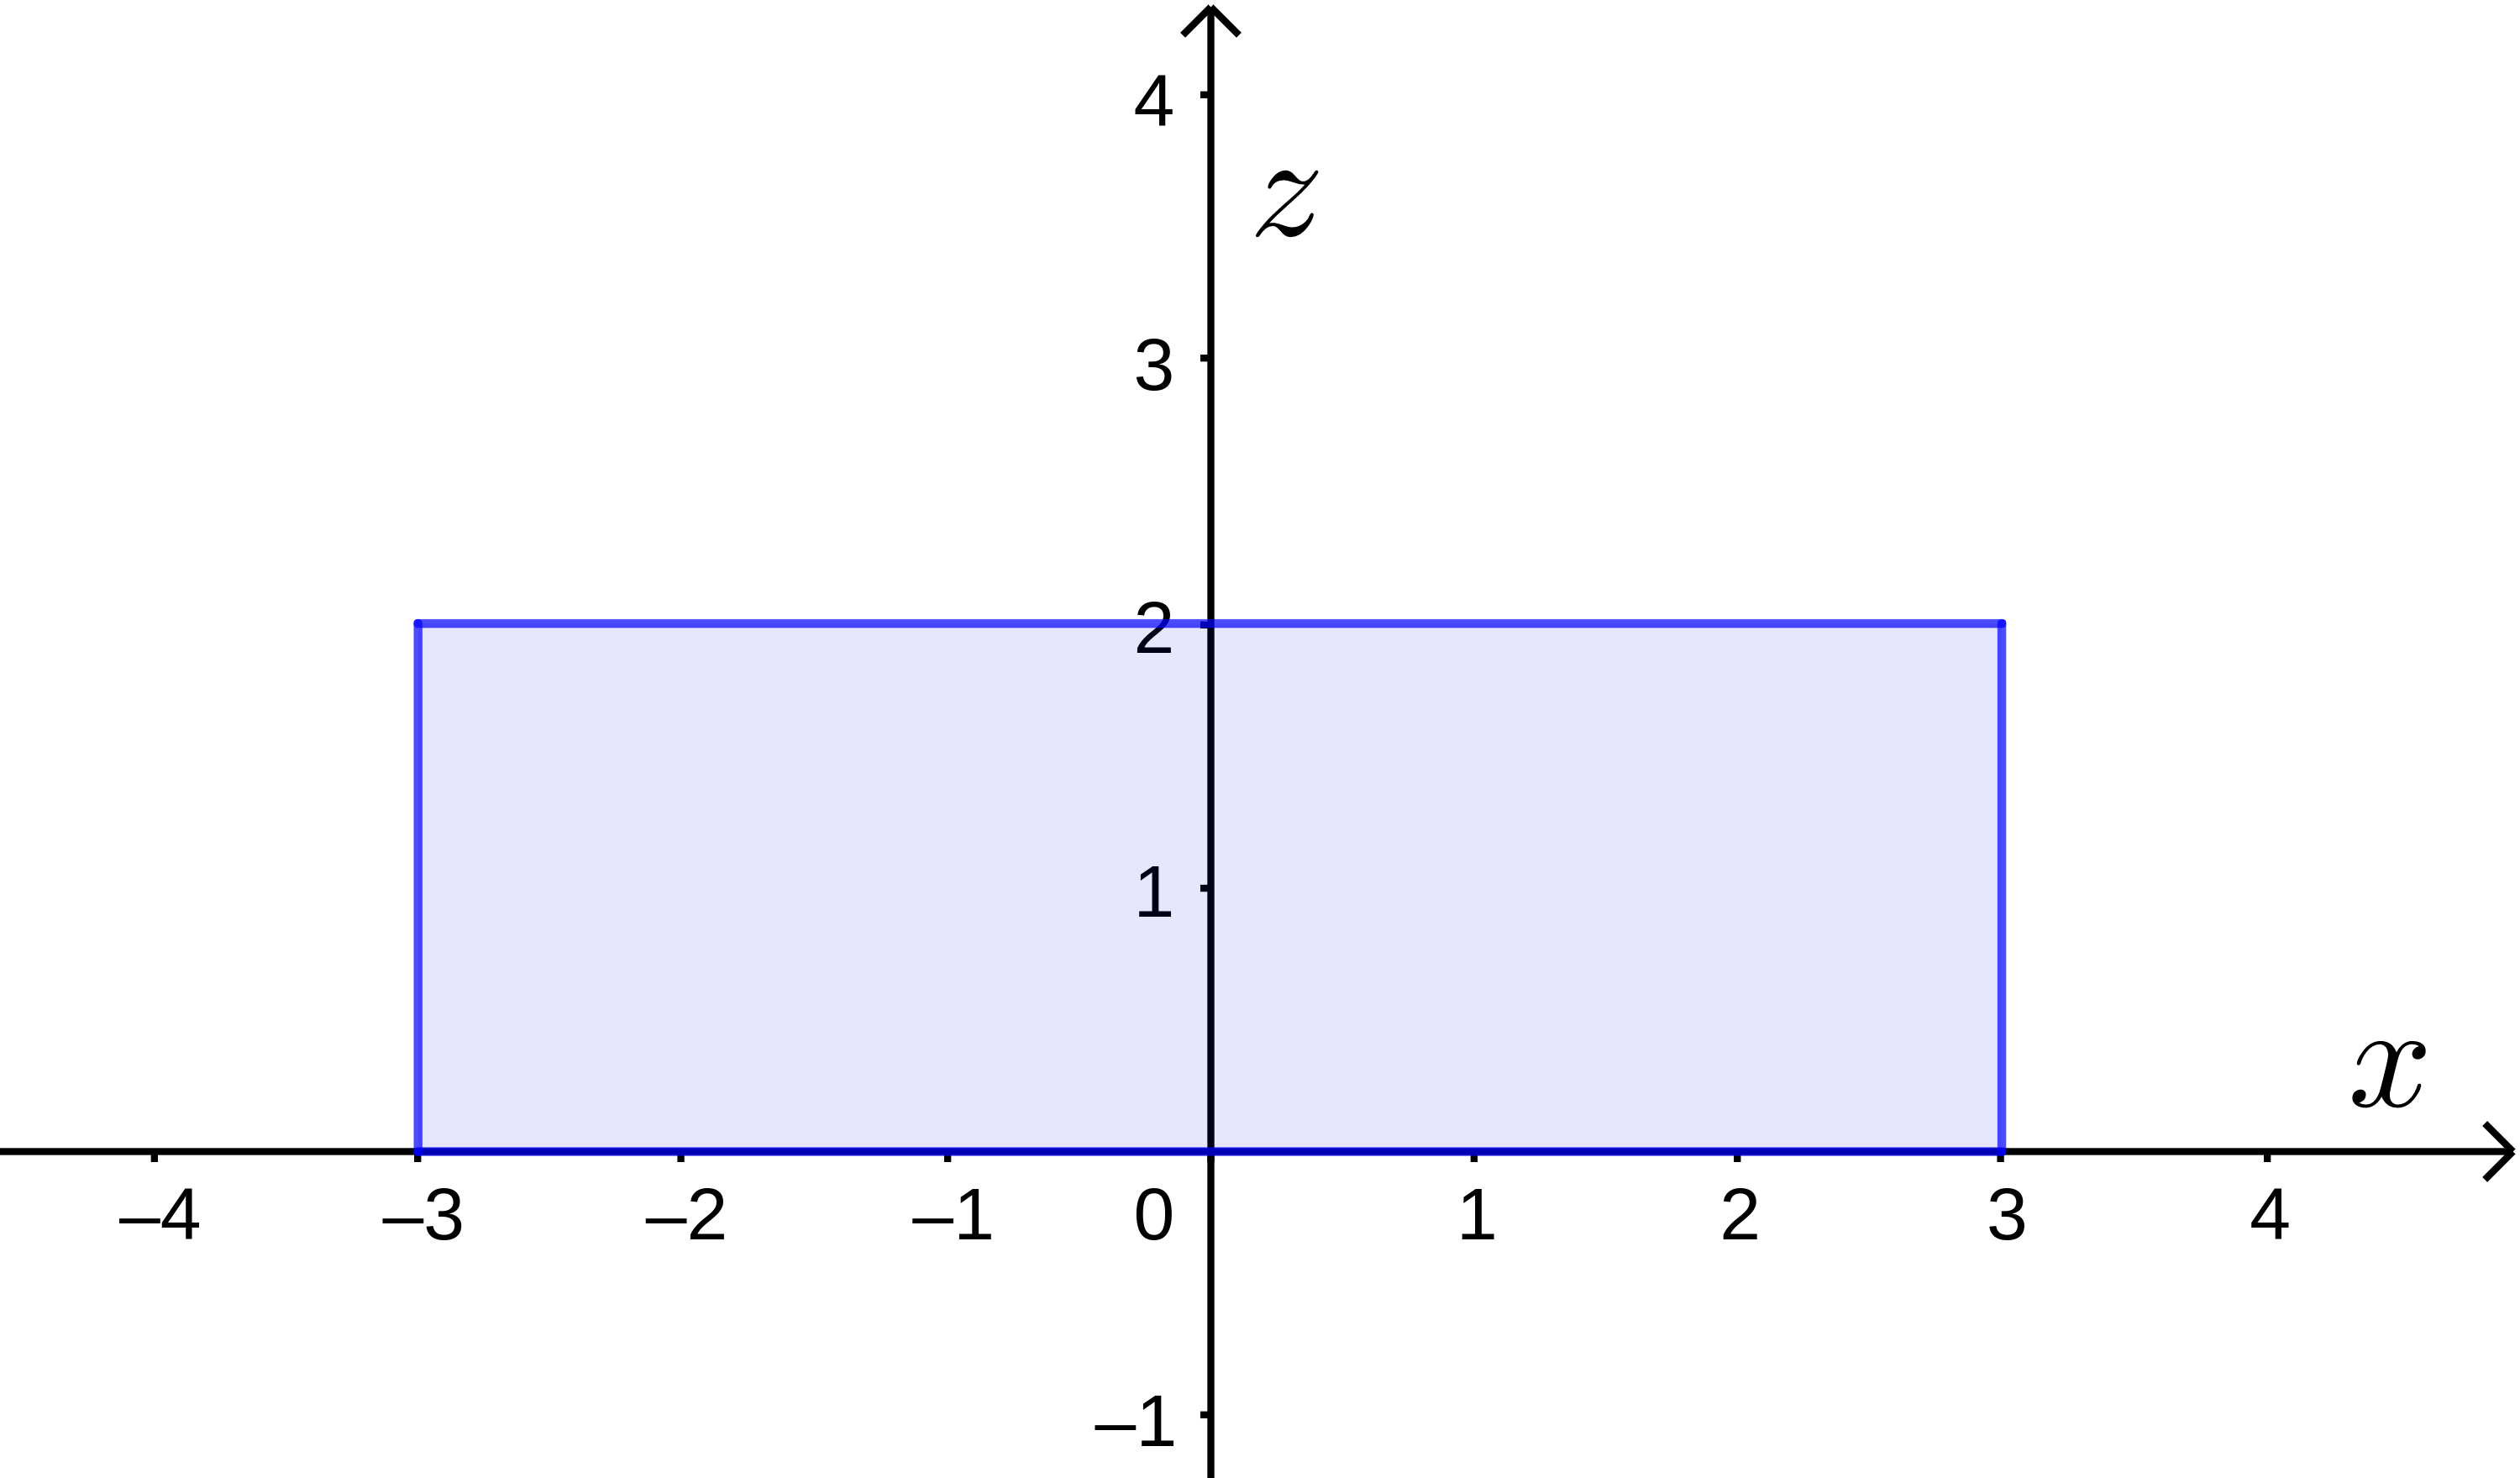
\includegraphics[width=6cm]{img/5a.png}
                \end{center}
                Escribimos la ecuación para $y=g(x,z)=\sqrt{9-x^2}$, entonces
                $\displaystyle g_x(x,z)=\frac{x}{\sqrt{9-x^2}}$ y
                $\displaystyle g_z(x,z)=0$

                Aplicando el teorema para convertir la integral de superficie
                en una integral doble
                \[
                    \displaystyle \iint_{S}{f(x,y,z)\,dS}
                    =\iint_{D}{
                        f(x,g(x,z), z)
                        \sqrt{\left[g_x(x,z)\right]^2+\left[g_z(x,z)\right]^2+1}
                    \,dA}
                \]
                Entonces tendremos que
                \begin{align*}
                    \iint_{S}{f(x,y,z)\,dS}
                    &= \iint_{D}{\left(
                        x^2 \sqrt{9-x^2}+z^2
                    \right)
                    \sqrt{
                        \frac{x^2}{9-x^2}+1
                    }
                    \,dA}\\[.3cm]
                    &= \int_{-3}^{3}{
                        \int_{0}^{2}{
                            \left(
                                3x^2+\frac{3z^2}{\sqrt{9-x^2}}
                            \right)
                        \,dz}
                    \,dx}\\[.3cm]
                    &= \int_{-3}^{3}{
                        \left[
                            3x^2z+\frac{z^3}{\sqrt{9-x^2}}
                        \right]_{0}^{2}
                    \,dx}\\[.3cm]
                    &= \int_{-3}^{3}{
                        \left(
                            6x^2+\frac{8}{\sqrt{9-x^2}}
                        \right)
                    \,dx}\\[.3cm]
                    &= \left[
                        2x^3+8\sen^{-1}{\left(\frac{x}{3}\right)}
                    \right]_{-3}^{3}\\
                    &= 108 + 8\pi
                \end{align*}
            }

            \item{
                $f(x,y,z) = x^2yz$ y $S$ la parte del plano $z = 1 + 2x + 3y$
                que está arriba del rectángulo $[0,3] \times [0,2]$

                \color{azul}
                % Respuesta
                Se entiende que la región $D = [0,3] \times [0,2]$, es la
                proyección acotada del plano $S$ sobre el plano $xy$, o sea que
                $x\in[0,3]$ e $y\in[0,2]$.

                Sea $z=g(x,y)$, entonces $g_x(x,y)=2$ y $g_y(x,y)=3$. Ahora
                aplicamos el teorema
                \begin{align*}
                    \iint_{S}{f(x,y,z)\,dS}
                    &= \iint_{D}{
                        f(x,y,g(x,y))
                        \sqrt{
                            \left[g_x(x,y)\right]^2+\left[g_y(x,y)\right]^2+1
                        }\,dA}\\[.2cm]
                    &= \int_{0}^{2}{
                        \int_{0}^{3}{
                            x^2y\left(1+2x+3y\right)
                            \sqrt{4+9+1}
                        \,dx}
                    \,dy}\\[.2cm]
                    &= \sqrt{14}\int_{0}^{2}{
                        \int_{0}^{3}{
                            \left(x^2y+2x^3y+3x^2y^2\right)
                        \,dx}
                    \,dy}\\[.2cm]
                    &= \sqrt{14}\int_{0}^{2}{
                        \left[
                            \frac{x^3y}{3}+\frac{x^4y}{2}+x^3y^2
                        \right]_{0}^{3}
                        \,dy}\\[.2cm]
                    &= \sqrt{14}\int_{0}^{2}{
                        \left(
                            9y+\frac{81}{2}y+27y^2
                        \right)
                    \,dy}\\[.2cm]
                    &=\sqrt{14}\left[
                        \frac{99}{4}y^2+9y^3
                    \right]_0^2\\
                    &= 71\sqrt{14}
                \end{align*}
            }
            \end{enumerate}


	    }

        % Ejercicio 6
        \item {
           Calcular $\displaystyle\iint_{S} \mathbf{F} \cdot d \mathbf{S}$

            \begin{enumerate}
            \item{
                $\mathbf{F} (x,y,z) = (0,y,-z)$ y $S$ consiste en el paraoloide
                $y = x^2 + z^2$, $0 \leq y \leq 1$, y el disco
                $x^2 + z^2 \leq 1$, $y = 1$

			\color{azul}
            % Respuesta
            Sean $S_1$ la superficie del paraboloide y $S_2$ la superficie del disco, entonces
            $$ \iint_{S} \mathbf{F} \cdot d \mathbf{S}
            = \iint_{S_1} \mathbf{F} \cdot d \mathbf{S}
            + \iint_{S_2} \mathbf{F} \cdot d \mathbf{S} $$

            Para $S_1$: $\bar{\Phi}(u,v)=\left(u, u^2+v^2, v\right)$
            $$ \bar{T}_u(u,v)=\left(1, 2u, 0\right) $$
            $$ \bar{T}_v(u,v)=\left(0, 2v, 1\right) $$
            $$ (\bar{T}_u \times \bar{T}_v)(u,v)=\left(2u, -1, 2v\right) $$
            $$ \mathbf{F}(\bar{\Phi}(u,v)) = \left(0, u^2+v^2, -v\right)$$
            entonces
            \begin{align*}
                \iint_{S_1} \mathbf{F} \cdot d \mathbf{S}
                &= \iint_D{(0, u^2+v^2, -v)\cdot(2u, -1, 2v)\,dA}\\[.2cm]
                &= \iint_D{(-u^2-v^2-2v^2)\,dA}
            \end{align*}
            Tomamos a $D$ como la proyección del paraboloide en el plano $xz$, que es un círculo de radio $1$, haciendo el cambio de coordenadas a polares tendremos
            \begin{align*}
                &= \int_{0}^{2\pi}{
                    \int_{0}^{1}{
                        -(r^2+2r^2\sen^2{\theta})r
                    \,dr}
                \,d\theta}\\[.2cm]
                &= \int_{0}^{2\pi}{
                    \int_{0}^{1}{
                        (-r^3)(1+2\sen^2{\theta})
                    \,dr}
                \,d\theta}\\[.2cm]
                &= \int_{0}^{2\pi}{
                    (1+2\sen^2{\theta})
                \,d\theta}
                \cdot
                \int_{0}^{1}{
                    (-r^3)
                \,dr}\\[.2cm]
                &= (4\pi)\left(-\frac{1}{4}\right)\\
                &= -\pi
            \end{align*}

            Para $S_2$: $\bar{\Psi}(r,\theta)=(r\cos{\theta}, 1, r\sen{\theta})$ con $0\leq r\leq 1$ y $0\leq\theta\leq 2\pi$
            $$ \bar{T}_r=(\cos{\theta}, 0, \sen{\theta}) $$
            $$ \bar{T}_\theta=(-r\sen{\theta}, 0, r\cos{\theta}) $$
            \begin{align*}
                (\bar{T}_r \times \bar{T}_\theta)(u,v)
                &= (0, -r\cos^2{\theta}-r\sen^2{\theta}, 0)\\
                &= (0, -r, 0)
            \end{align*}
            $$ \mathbf{F}(\Psi(r,\theta)) = (0,1,-r\sen{\theta}) $$
            entonces
            \begin{align*}
                \iint_{S_2}{\mathbf{F}\cdot d\mathbf{S}}
                &= \iint_{D}{
                    (0,1,-r\sen{\theta})
                    \cdot
                    (0, -r, 0)
                \,dA}\\[.2cm]
                &= \iint_{D}{-r\,dA}\\[.2cm]
                &= -\int_{0}^{2\pi}{
                    \int_{0}^{1}{
                        r
                    \,dr}
                \,d\theta}\\[.2cm]
                &= (-2\pi)\left(\frac{1}{2}\right)\\
                &= -\pi
            \end{align*}

            Por lo tanto
            $$ \iint_{S} \mathbf{F} \cdot d \mathbf{S}
            = \iint_{S_1} \mathbf{F} \cdot d \mathbf{S}
            + \iint_{S_2} \mathbf{F} \cdot d \mathbf{S}
            = (-\pi)+(-\pi) = -2\pi$$
            }

            % 6b
            \item{
            	$\mathbf{F} (x,y) = (xze^y,-xze^y,z)$ y $S$ la parte del plano $x + y+ z = 1$ en el primer octante con orientación hacia arriba

           \color{azul}
            % Respuesta
            La superficie $S$ se muestra a continuación
            \begin{center}
                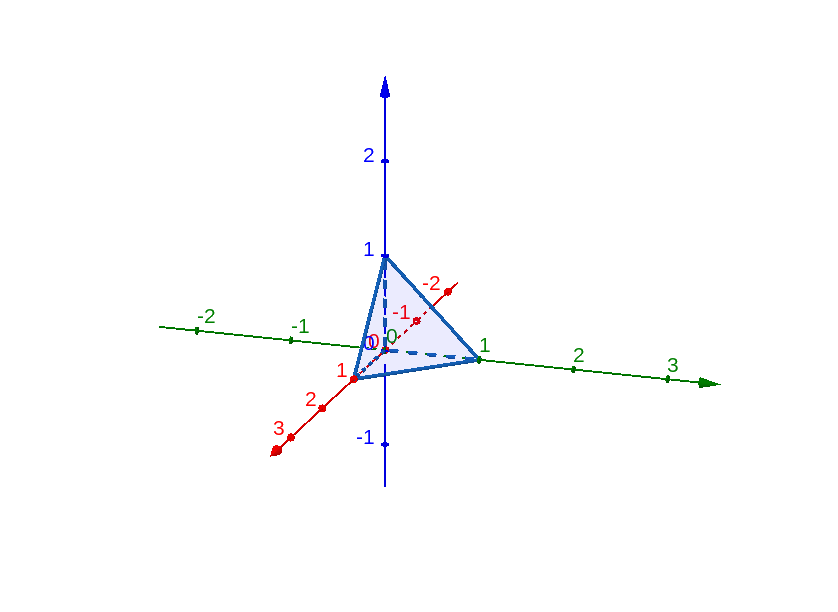
\includegraphics[width=10cm]{img/6b.png}
            \end{center}
            Tenemos que $z=1-x-y$, entonces $\bar{\Phi}(u,v) = (u,v,1-u-v)$ con $u,v\in[0,1]$
            $$ \bar{T}_u = (1,0,-1) $$
            $$ \bar{T}_v = (0,1,-1) $$
            $$ (\bar{T}_u\times\bar{T}_v)(u,v) = (1,1,1) $$
            \begin{align*}
                \mathbf{F}(\bar{\Phi}(u,v))
                &= \left(
                    u(1-u-v)e^v,
                    -u(1-u-v)e^v,
                    1-u-v
                \right)\\
                &= \left(
                    -(u^2-u+uv)e^v,
                    (u^2-u+uv)e^v,
                    1-u-v
                \right)
            \end{align*}
            Entonces
            \begin{align*}
                \iint_{S} \mathbf{F} \cdot d \mathbf{S}
                &= \iint_{D}{
                    \left(-(u^2-u+uv)e^v,(u^2-u+uv)e^v,1-u-v\right)
                    \cdot
                    (1,1,1)
                \,dA}\\[.2cm]
                &= \iint_D{
                    (1-u-v)
                \,dA}\\[.2cm]
                &= \int_{0}^{1}{
                    \int_{0}^{1}{
                        (1-u-v)
                    \,du}
                \,dv}\\[.2cm]
                &= \int_{0}^{1}{
                    \left[
                        u-\frac{1}{2}u^2-uv
                    \right]_{0}^{1}
                \,dv}\\[.2cm]
                &= \int_{0}^{1}{
                    \left(
                        \frac{1}{2}-v
                    \right)
                \,dv}\\[.2cm]
                &= \left[
                    \frac{1}{2}v-\frac{1}{2}v^2
                \right]_{0}^{1}\\
                &= 0
            \end{align*}
            }
            \end{enumerate}


        }

        % Ejercicio 7
        \pagebreak
        \item {
            Usar el teorema de Stokes para evaluar $\displaystyle\iint_{S} \nabla \times \mathbf{F} \cdot d\mathbf{S}$, donde $\mathbf{F}(x,y,z) =(x^2y^3z,\sin(xyz),xyz)$ y $S$ es la parte del cono $y^2 = x^2 + z^2$ que está entre los planos $y = 0$ y $y = 3$ orientada en dirección positiva del eje Y.

            \color{azul}
            Sabemos que la frontera de S es una curva orientable y cerrada por
            como está definida. También podemos ver que las primeras derivadas
            de F son continuas y que D(la parametrización de la superficie en
            $\mathbb{R}^2$) es una región elemental, por lo tanto podemos
            aplicar el teorema de Stokes.

            El teorema dice que:

            $\iint_{S} \nabla \times \mathbf{F} \cdot d\mathbf{S} = \int_{\mathcal{C}} \mathbf{F} \cdot d\mathbf{l}$

            La curva $\mathcal{C}$ será la frontera de la superficie S y la parametrizaremos del siguiente modo: $\sigma(t) = (\cos(t), 3, \sin(t))$ con $t \in [0, 2\pi]$

            Ahora obtenemos $d\mathbf{l} = (dx, dy, dz) = (-\sin(t), 0, \cos(t))$

        Componemos F con $\sigma(t)$ y tenemos que:

        $\int_{\mathcal{C}} \mathbf{F} \cdot d\mathbf{l} = \int_{0}^{2\pi} (-27\cos^2(t)\sin^2(t) + 0 + 3\cos^2(t)\sin(t)) dt$

        Resolvemos la integral dividendola en dos:

         $\int_{\mathcal{C}} \mathbf{F} \cdot d\mathbf{l} = \int_{0}^{2\pi} -27\cos^2(t)\sin^2(t) dt +   \int_{0}^{2\pi}3\cos^2(t)\sin(t)dt$

         Usamos la identidad trigonométrica $\cos^2(t)\sin^2(t) = \frac{1 - \cos(4t)}{8}$ y tenemos que:
         \begin{align*}
                \int_{0}^{2\pi}{-27\cos^2(t)\sin^2(t)dt}
                &= -\frac{27}{8} \int_{0}^{2\pi}{(1 - \cos(4t)) dt}
                = -\frac{27}{8} \Big(\int_{0}^{2\pi}{(1)dt }  - \int_{0}^{2\pi}{\cos(4t)dt}\Big)\\[0.3cm]
                &= -\frac{27}{8}\Big((t - \frac{1}{4} \sin(4t))\Big |_{0}^{2\pi}\Big)
                = -\frac{27}{8} (2\pi - 0)
               	= -\frac{27}{4}\pi
            \end{align*}

		Resolvemos la otra integral:
		\begin{align*}
                &\int_{0}^{2\pi}{3\cos^2(t)\sin(t)dt}
                = -3\Big( \frac{\cos^3(t)}{3}\Big |_{0}^{2\pi}\Big)
                = -3 \Big(-\frac{1}{3} + \frac{1}{3}\Big)
               	= -3 (0)
               	= 0
            \end{align*}

		De ahí, tenemos que:
		$\int_{\mathcal{C}} \mathbf{F} \cdot d\mathbf{l} = -\frac{27}{4}\pi + 0 = -\frac{27}{4}\pi$

		Por lo tanto:

		$\iint_{S} \nabla \times \mathbf{F} \cdot d\mathbf{S} = -\frac{27}{4}\pi$

        }

        % Ejercicio 8
        \item {
            Usar el teorema de Gauss para evaluar $\displaystyle\iint_{S} \mathbf{F} \cdot d\mathbf{S}$, con $\mathbf{F}(x,y,z) = (x^3y,-x^2y^2,-x^2yz)$ y $S$ la superficie cerrada definida por el hiperboloide $x^2 + y^2 - z^2 = 1$ y los planos $z = -2$ y $z = 2$

            \color{azul}
            Sabemos que el hiperboloide es una región elemental por como está definido. Podemos ver que S (la frontera de la hiperboloide), es cerrada y orientable. También podemos ver que las primeras derivadas de F son continuas, por lo tanto podemos aplicar el teorema de Gauss.

            El teorema dice que:

            $\iint_{S} \mathbf{F} \cdot d\mathbf{S} = \iiint_{W} \nabla \cdot \mathbf{F} d\mathbf{V}$

            Obtenemos $\nabla \cdot \mathbf{F} = 3x^2y - 2x^2y - x^2y = 0$

            Entonces tenemos que:

             $\iint_{S} \mathbf{F} \cdot d\mathbf{S} = \iiint_{W} \ 0 \  d\mathbf{V}$

            No necesitamos parametrizar W para ver que el resultado de esa integral será cero.

            Por lo tanto:

            $\iint_{S} \mathbf{F} \cdot d\mathbf{S} = 0$



        }

         % Ejercicio 9
        \item {
            Usar propiedades del rotacional para mostrar que
            \[
                \int_{\mathcal{C}} {{\left(f \nabla g + g \nabla f\right)} \cdot d\mathbf{l}} = 0
            \]
            \color{azul}
            Esta afirmación es falsa. Veamos un contraejemplo.\\
            Sea $g(x, y, z) = f(x, y, z) = x$ y $c(t) = (t, 0, 0) t\in [0, 1]$ la
            curva parametrizada.
            Entonces la integral es
            \begin{align*}
                \int_{\mathcal{C}}{x(1, 0, 0) + x(1, 0, 0)dl} &= \int_{\mathcal{C}}{(2x, 0, 0)dl}
                = \int_{0}^{1}{(2t, 0, 0)\cdot (1, 0, 0)dt} \\
                &= \int_{0}^{1}{2tdt}  = t^{2} \Big |_{0}^{1} = 1^{2} - 0^{2} \\
                &= 1 \neq 0
            \end{align*}
            Pero supongamos que $\mathcal{C}$ es una curva orientable y cerrada,
            que $fg$ tiene sus primeras derivadas continuas y que la
            superficie englobada por $\mathcal{C}$ es orientable y su dominio es
            una región elemental con frontera cerrada.\\
            Tomando las condiciones válidas, vemos que cumple el teorema de Stokes.

            \begin{align*}
                \int_{\mathcal{C}} {{\left(f \nabla g + g \nabla f\right)}\ \cdot d\mathbf{l}}
				&= \int_{\mathcal{C}} \left(f \left(\frac{\partial}{\partial x} g,\ \ \frac{\partial}{\partial y}g,\ \ \frac{\partial}{\partial z}g\right) + g \left(\frac{\partial}{\partial x} f,\ \ \frac{\partial}{\partial y}f,\ \ \frac{\partial}{\partial z}f\right)\right) \cdot d\mathbf{l} &\mathrm{(Definicion \ nabla)}\\
				&=\int_{\mathcal{C}}\left(f\frac{\partial}{\partial x} g + g\frac{\partial}{\partial x} f ,\ \ f \frac{\partial}{\partial y} g + g\frac{\partial}{\partial y} f ,\ \ f \frac{\partial}{\partial z} g + g \frac{\partial}{\partial z} f \right) \cdot d\mathbf{l} & \mathrm{(Agrupando)}\\
                &= \int_{\mathcal{C}}\left(\frac{\partial}{\partial x} fg,\ \ \frac{\partial}{\partial y}fg,\ \ \frac{\partial}{\partial z}fg\right) \cdot d\mathbf{l} &\mathrm{(Regla \ del \  Producto)}\\
&=\int_{\mathcal{C}}(\nabla(fg)) \cdot d\mathbf{l} &\mathrm{(Definicion \ nabla)}\\
&=\iint_{S} (\nabla \times \nabla(fg)) \cdot dS &\mathrm{(Teorema \ de \ Stokes)}\\
&=\iint_{S} 0 \cdot dS &\mathrm{(Propiedades \ del \ Rotacional)}\\
&= 0 &\mathrm{(Definicion \ Integral)}
            \end{align*}



        }
    \end{enumerate}
\end{document}
